\documentclass{book}

\usepackage[margin=1in]{geometry}
\usepackage{amsmath,amssymb, amsthm}

\usepackage{microtype}
\usepackage{tikz}
	\usetikzlibrary{positioning}\usetikzlibrary{arrows}
	\tikzset{every edge/.style={ % Sets the properties for each transition	1
			draw,
			->,
			auto,
			very thick}}

\DeclareMathOperator*{\argmax}{arg\,max}
\DeclareMathOperator*{\argmin}{arg\,min}
\DeclareMathOperator*{\E}{\mathbb E}

\usepackage{parskip}

\newcommand\Tstrut{\rule{0pt}{5.6ex}}         % = `top' strut
\newcommand\Bstrut{\rule[-0.9ex]{0pt}{0pt}}   % = `bottom' strut

\newcommand\geqc{\succcurlyeq}

\setlength{\skip\footins}{1cm}
\setlength{\footnotesep}{0.4cm}

\begin{document}
	\chapter{Examples}
	
	\section{Wrong Variables.}
	Suppose worlds are parameterized by three variables $A, B, C$, each of which can take on two values: variable $A$ can take on either $a$ or $\bar a$, $B$ can take on $b$ or $\bar b$, and $C$ is either $c$ or $\bar c$.
	
	Suppose further that the original agent cannot observe these variables directly, but rather observes variables $X$ and $Y$, which are logically defined as 
	\begin{align*}
		X &:= A \land B \\
		Y &:= B \lor C
	\end{align*}
	
	and that I originally have a preference order
	\[ x \bar y \geqc \bar x y \geqc \bar x \bar y \geqc x y  \]
	
	The variables $X$ and $Y$ are perfectly well-defined, and don't vary with time\footnote{which is already more than can be said for most variables that people care about --- for example, `nutritious', `inoffensive', and `affluent' are all moving targets}, and yet still it may be that there is a good reason to change preferences after changing the structure of your beliefs.
	
	
	
	\begin{center}
		\begin{tabular}{cccc}
			$x \bar y $ & $\bar x y$ & $\bar x \bar y$ & $x y$ \\\hline
			\rule{0pt}{2.3em}$\varnothing$ & \parbox[c]{0.5cm}{$\bar a b \bar c$\\$\bar a b c$ \\ $a \bar b c$} 
				& \parbox[c]{0.5cm}{$\bar a \bar b \bar c$ \\ $a \bar b \bar c$}
				& \parbox[c]{0.5cm}{$abc$} \\[1.3em]\hline
		\end{tabular}
	\end{center}
	\vspace{1em}
	
	
	There are two intuitions that one might have. The first, and the one that jives best with the utility-maximization perspective, is that even seeing the world from this new perspective, your preferences really ought to be thought of as over the variables you observe ($X$ and $Y$). After all, discovering that you have actually been referring to many chemically distinct solutions as ``water'' should not necessarily cause you to disassociate them, or modify your 
	
	If the preference order I gave above was truly what you had preferences for (and not merely that you were mistaken about what you enjoyed), then it does not matter what you discover about the world --- as far as you are concerned, the utility of a world parameterized by $A,B,C$ is determined purely by its effect on $X$ and $Y$. 
	
	This results in the following total pre-order:
	
	\[ \left\{~\parbox[c]{0.5cm}{$\bar a b \bar c$\\$\bar a b c$ \\ $a \bar b c$}~\right\} \geqc \left\{~\parbox[c]{0.5cm}{$\bar a \bar b \bar c$ \\ $a \bar b \bar c$}~\right\} \geqc \left\{abc \right\} \]
	
	The second intuition that one might have, is that you have been blind to the differences between certain worlds and have accidentally been conflating them. 
	
	
	 the reason that one had decided, for instance, that $\bar x y \geqc \bar x \bar y$, is that the vast majority of the occurrences of worlds matching $\bar x y$ are in fact $\bar a b \bar c$, whereas 
	
	
	\section{New Constraint}
	
	\section{Gamification}
	Gamification induce some intrinsic value into 
	
	From one perspective, this is an obvious part of the application of expected utility for decision making --- it is common for modelers to say things along the lines of ``by playing this game, I will get a(n expected) payoff of $g$ utils'', in the same sense that one would gain utility by watching a film or spending time with friends; these are simply regarded as atomic pleasure
	
	I posit that it is worth looking into the reasons that this is the case.
	
	\section{Value Capture}
	
	
	\section{Cultural Revolution}
	
	
%	You, however, not being able to observe the world, have preferences for $C := A \otimes B$, for $D := B \otimes C$, and also for $E := C \otimes A$, amounting to a choice of exactly one out of every pair of real variable. All three conjunctions are, of course, unsatisfiable.
	

	\chapter{Context}
	From a a modeling perspective, what can be said to determine [a person]'s actions? Why do [people] do things? These are some of the central questions in behavioral economics. 
	
	
	\begin{center}\scshape\color{blue}\selectfont
		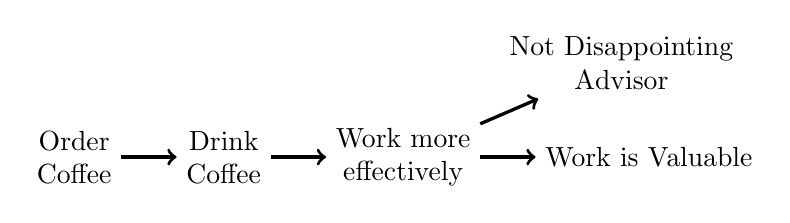
\begin{tikzpicture}[align=center]
			\node (O) {Order \\ Coffee};
			\node [right=2em of O] (C) {Drink \\ Coffee};
			\node [right=2em of C] (W) {Work more \\effectively};	
			\node [above right=1em of W] (A) {Not Disappointing\\ Advisor};
			\node [right=2em of W] (I) {Work is Valuable};
			
			\draw (O) edge (C) (C) edge (W) (W) edge (A) (W) edge (I);
		\end{tikzpicture}
	\end{center}
	
	The chain of rational reasons then bottoms out with some desire, moral, preference, which is not itself the kind of thing that can be interrogated with the question ``why'', in the same way. Sure, there may be a causal explanation for why it came to be that you enjoy coffee, but that is not the 
	
	
			
	A policy
	\[ \pi: \mathrm{States} \to \mathrm{Actions} \]
	
%	If $S$ is a set of states, and $O$ is the set of outcomes, 
	
%	let $\mathcal L$
	
	% By Savage, we know that we don't need to assumsemithicke the existence of a probability distribution (over states or outcomes); one can derrive this from the axioms
	
	\section{The Emotion / Reason Dichotomy}
	Morals, preferences, goals, utilities, rewards/punishments, and desires all have something in common: the behavior that characterizes them is an optimization. They answer a question about \emph{why} something was done, in a way that is compatible with planning and rational, well-thought-out behavior. If one sees a person repeatedly doing something, say walking their dog, it is reasonable to conclude that either they hold that this is a morally good thing to do, have a preference or goal / sub-goal of walking their dog, enjoy it, or have times when they want to do it. Moreover, these are considered explanations of \emph{why} behavior happens. They are descriptions of the things that agents optimize.
	
	The second feature they share is a subjectivity: anyone can have any preferences or utilities or rewards (perhaps subject to certain constraints if you don't want to be manipulated, want to behave robustly in the presence of adversaries, and so on). Once the space has been constrained, having different preferences is merely... a matter of preference. The theories we use for modeling agents do not take into account the mechanisms by which one might obtain preferences, which 
	
	More egregiously still, standard utility / reward maximization picture has nothing to say about the possibility of these quantities changing over time.
	
	
	
	All of this is to be contrasted with two other concepts:

	\begin{enumerate}
		\item Empirical analysis which determines that some behavior (as opposed to another one) is occurring. 
		\item Theories of belief, rationality, and \emph{how} to optimize.
	\end{enumerate}
	
	
	
	All of these have been postulated as reasons why people do things, and more generally, as theories about ways to shape behavior of agents. 
	
	
	
	The general idea is to consider two descriptions of motivation equivalent if they necessarily result in indistinguishable behavior. 
	
	% Related: opinions --- beliefs + judgement
	% 	Emotions --- attitudes towards things [mroe general]
	
	\subsection{Utilities and Preferences}
	
	To simplify things, economists and decision theorists start with the case when the set of possibilities is small and finite. If $O$ is the set of things one could choose between, i.e., the set of outcomes, then we can formalize a preference as a pre-order $(O, \preccurlyeq)$ on $O$.
	
	\begin{align*}
		\forall x \in O.&~x \preccurlyeq x \tag{Reflexivity}\\
		\forall x,y,z \in O.&~(x\preccurlyeq y)~\land~( y \preccurlyeq z) \Rightarrow~(x \preccurlyeq z) \tag{Transitivity}
	\end{align*}
	
	Rather than dealing with the partial order directly, we might like to have an embedding into something we have more intuition for, such as natural numbers or a continuous space. The problem with this, of course, is that the space may have some structure which is incompatible with the partial order. 
	
	of these results in a ranking, 
	
	However, there is often a lot more structure on outcomes
	
	
	

	
	\subsection{Utilities and Rewards}
	
	Both utilities and rewards are real-valued functions from something in the world to a one-dimensional notion of `good-ness' represented by $\mathbb R$, and hence are sometimes thought of as equivalent; here we will do some of the work to explore in what sense they might be equivalent, and the sorts of issues that might come up if conflating the two without any thought.
	
	Utilities are over outcomes, so a utility function $U : Z \to \mathbb R$ must be
	
	\[ \pi^*(x) = \argmax_{y: Y} \E_{z : Z} \Big[ U(z)~\Big|~ y,x\Big] \]
	
	\subsubsection{Determinism}
	If $\cal W$ is the set of all possible world states, and $\tau: \cal W \to W$ is a deterministic function describing the evolution of the world, then having a preference over futures starting at $w_0$ and consistent with $\tau$ is meaningless, as there is only one such sequence of worlds. Therefore, pure determinism only makes sense with agents with imperfect information. 
	
	Let $X$ be the space of world representations for an agent, and let $\eta: \mathcal W \to X$ be some function, thought of as perception, which generates a world representation. This gives us an equivalence class $[w] := \eta^{-1}(\eta(w))$ of information sets of the agent, which may not be stable under $\tau$, and so it may be the case that $w \underset\eta\sim w'$ but not $\tau(w) \underset\eta\sim \tau(w')$
	
	
	
	The fact that one gets more information over time suggests that the optimal policy, even with infinite computation, in general will change with additional samples. After two steps, the policy becomes
	
	\begin{align*}
		\pi^*(\eta\circ\tau (x)) &= \argmax_{y: Y} \E_{z : Z} \Big[ U(z)~\Big|~ y,\eta\tau x \Big]  \\
			&= \argmax_{y: Y} \int\limits_{\mathrm dZ} \Pr\Big[z~\Big|~\left(Y^{(t)} = y \right) \land \left(X^{(t)}= \eta \circ \tau (x)\right) \land \left(X^{(t-1)} = x \right) \Big] U(z)
	\end{align*}
		
	
	\subsubsection{Nondeterminism}
	Once again, suppose $\cal W$ is the set of possible worlds, with now $\tau: \mathcal W \to 2^{\mathcal W}$, a non-deterministic version of the transition function in the deterministic setting from before.
	
	In this more general case, we can still relate the two. To begin, suppose that we have a complete preferences over possible futures. 
	
	
	\section{Fields in which a related problem has been addressed}
	
%	\subsection{Selective Pressure}
	\subsection{Art History} % Model literally changes in peoples' aesthetic preferences
	\subsection{Pedagogy} % Representation Changes.
	\subsection{}
	
	
	\section{Applications}
	
	\subsection{Content Recommendation}
	The way that these assumptions of static preferences manifest themselves in content recommendation systems is the
	
	\subsection{AI Safety}
	\subsection{Better Inverse Reinforcement Learning}
	\subsection{Robotics: Life-long Learning}
	\subsection{Meta Ethics}
	
	\section{As a Learning Problem}
	
	
\end{document}